% ACAPE: measured evaluation of runtime parameter adaptation for fq_codel
%
% Every numeric result in this document is \input{} from files generated by
% src/analyse.py directly from the experiment logs. No figure in the prose is
% typed by hand. Rebuild with:
%   python3 src/analyse.py --results results --outdir paper/generated
%   pdflatex acape.tex
\documentclass[conference]{IEEEtran}
\IEEEoverridecommandlockouts

\usepackage{cite}
\usepackage{amsmath,amssymb}
\usepackage{graphicx}
\usepackage{booktabs}
\usepackage{url}
\usepackage{xcolor}
\usepackage[hidelinks]{hyperref}

\graphicspath{{generated/}{../figures/}{../figures/steps/}{../figures/comparison/}{../figures/runs/}}
% GENERATED by src/analyse.py -- do not edit by hand.
\newcommand{\CakeBacklogStaged}{10.47}
\newcommand{\CakeBacklogSteady}{6.673}
\newcommand{\CakeBulkRttMeanStaged}{30.13}
\newcommand{\CakeBulkRttMeanSteady}{33.65}
\newcommand{\CakeBulkRttPninetyfiveStaged}{37.05}
\newcommand{\CakeBulkRttPninetyfiveSteady}{37.41}
\newcommand{\CakeGoodputStaged}{9.24}
\newcommand{\CakeGoodputSteady}{9.414}
\newcommand{\CakeJainStaged}{1}
\newcommand{\CakeJainSteady}{0.9999}
\newcommand{\CakeProbeRttMeanStaged}{21.48}
\newcommand{\CakeProbeRttMeanSteady}{21.76}
\newcommand{\CakeProbeRttPninetyfiveStaged}{22.27}
\newcommand{\CakeProbeRttPninetyfiveSteady}{22.9}
\newcommand{\CodelBacklogStaged}{24.13}
\newcommand{\CodelBacklogSteady}{8.55}
\newcommand{\CodelBulkRttMeanStaged}{105.5}
\newcommand{\CodelBulkRttMeanSteady}{44.5}
\newcommand{\CodelBulkRttPninetyfiveStaged}{469.5}
\newcommand{\CodelBulkRttPninetyfiveSteady}{52.42}
\newcommand{\CodelGoodputStaged}{9.277}
\newcommand{\CodelGoodputSteady}{9.451}
\newcommand{\CodelJainStaged}{0.9911}
\newcommand{\CodelJainSteady}{0.9969}
\newcommand{\CodelProbeRttMeanStaged}{55.05}
\newcommand{\CodelProbeRttMeanSteady}{39.02}
\newcommand{\CodelProbeRttPninetyfiveStaged}{172}
\newcommand{\CodelProbeRttPninetyfiveSteady}{45.1}
\newcommand{\FqCodelAcapeBacklogStaged}{11.52}
\newcommand{\FqCodelAcapeBacklogSteady}{6.14}
\newcommand{\FqCodelAcapeBulkRttMeanStaged}{51.74}
\newcommand{\FqCodelAcapeBulkRttMeanSteady}{35.87}
\newcommand{\FqCodelAcapeBulkRttPninetyfiveStaged}{72.24}
\newcommand{\FqCodelAcapeBulkRttPninetyfiveSteady}{40.16}
\newcommand{\FqCodelAcapeGoodputStaged}{9.179}
\newcommand{\FqCodelAcapeGoodputSteady}{9.402}
\newcommand{\FqCodelAcapeJainStaged}{0.9999}
\newcommand{\FqCodelAcapeJainSteady}{1}
\newcommand{\FqCodelAcapeProbeRttMeanStaged}{22.25}
\newcommand{\FqCodelAcapeProbeRttMeanSteady}{22.5}
\newcommand{\FqCodelAcapeProbeRttPninetyfiveStaged}{24.15}
\newcommand{\FqCodelAcapeProbeRttPninetyfiveSteady}{24.43}
\newcommand{\FqCodelBacklogStaged}{11.28}
\newcommand{\FqCodelBacklogSteady}{6.79}
\newcommand{\FqCodelBulkRttMeanStaged}{51.99}
\newcommand{\FqCodelBulkRttMeanSteady}{36.39}
\newcommand{\FqCodelBulkRttPninetyfiveStaged}{72.71}
\newcommand{\FqCodelBulkRttPninetyfiveSteady}{40.56}
\newcommand{\FqCodelGoodputStaged}{9.235}
\newcommand{\FqCodelGoodputSteady}{9.414}
\newcommand{\FqCodelJainStaged}{1}
\newcommand{\FqCodelJainSteady}{0.9999}
\newcommand{\FqCodelProbeRttMeanStaged}{21.9}
\newcommand{\FqCodelProbeRttMeanSteady}{22.4}
\newcommand{\FqCodelProbeRttPninetyfiveStaged}{23.4}
\newcommand{\FqCodelProbeRttPninetyfiveSteady}{24.57}
\newcommand{\FqCodelShamBacklogStaged}{11.5}
\newcommand{\FqCodelShamBacklogSteady}{6.78}
\newcommand{\FqCodelShamBulkRttMeanStaged}{51.68}
\newcommand{\FqCodelShamBulkRttMeanSteady}{36.88}
\newcommand{\FqCodelShamBulkRttPninetyfiveStaged}{67.57}
\newcommand{\FqCodelShamBulkRttPninetyfiveSteady}{40.51}
\newcommand{\FqCodelShamGoodputStaged}{9.195}
\newcommand{\FqCodelShamGoodputSteady}{9.398}
\newcommand{\FqCodelShamJainStaged}{1}
\newcommand{\FqCodelShamJainSteady}{1}
\newcommand{\FqCodelShamProbeRttMeanStaged}{22.13}
\newcommand{\FqCodelShamProbeRttMeanSteady}{22.36}
\newcommand{\FqCodelShamProbeRttPninetyfiveStaged}{23.5}
\newcommand{\FqCodelShamProbeRttPninetyfiveSteady}{24.57}
\newcommand{\FqPieBacklogStaged}{18.61}
\newcommand{\FqPieBacklogSteady}{11.94}
\newcommand{\FqPieBulkRttMeanStaged}{101.8}
\newcommand{\FqPieBulkRttMeanSteady}{55.39}
\newcommand{\FqPieBulkRttPninetyfiveStaged}{214}
\newcommand{\FqPieBulkRttPninetyfiveSteady}{68.85}
\newcommand{\FqPieGoodputStaged}{9.223}
\newcommand{\FqPieGoodputSteady}{9.453}
\newcommand{\FqPieJainStaged}{0.9999}
\newcommand{\FqPieJainSteady}{1}
\newcommand{\FqPieProbeRttMeanStaged}{21.9}
\newcommand{\FqPieProbeRttMeanSteady}{22.04}
\newcommand{\FqPieProbeRttPninetyfiveStaged}{23.23}
\newcommand{\FqPieProbeRttPninetyfiveSteady}{23.27}
\newcommand{\PfifoBacklogStaged}{570.2}
\newcommand{\PfifoBacklogSteady}{789.2}
\newcommand{\PfifoBulkRttMeanStaged}{1586}
\newcommand{\PfifoBulkRttMeanSteady}{1753}
\newcommand{\PfifoBulkRttPninetyfiveStaged}{2366}
\newcommand{\PfifoBulkRttPninetyfiveSteady}{2372}
\newcommand{\PfifoGoodputStaged}{8.38}
\newcommand{\PfifoGoodputSteady}{9.453}
\newcommand{\PfifoJainStaged}{0.9862}
\newcommand{\PfifoJainSteady}{0.9957}
\newcommand{\PfifoProbeRttMeanStaged}{1153}
\newcommand{\PfifoProbeRttMeanSteady}{1711}
\newcommand{\PfifoProbeRttPninetyfiveStaged}{2318}
\newcommand{\PfifoProbeRttPninetyfiveSteady}{2344}
\newcommand{\PieBacklogStaged}{10.33}
\newcommand{\PieBacklogSteady}{8.84}
\newcommand{\PieBulkRttMeanStaged}{119.2}
\newcommand{\PieBulkRttMeanSteady}{47.29}
\newcommand{\PieBulkRttPninetyfiveStaged}{580.9}
\newcommand{\PieBulkRttPninetyfiveSteady}{61.9}
\newcommand{\PieGoodputStaged}{9.223}
\newcommand{\PieGoodputSteady}{9.413}
\newcommand{\PieJainStaged}{0.9614}
\newcommand{\PieJainSteady}{0.9959}
\newcommand{\PieProbeRttMeanStaged}{40.4}
\newcommand{\PieProbeRttMeanSteady}{39.14}
\newcommand{\PieProbeRttPninetyfiveStaged}{48.57}
\newcommand{\PieProbeRttPninetyfiveSteady}{46.93}
\newcommand{\RedBacklogStaged}{21.81}
\newcommand{\RedBacklogSteady}{26.68}
\newcommand{\RedBulkRttMeanStaged}{88.91}
\newcommand{\RedBulkRttMeanSteady}{82.65}
\newcommand{\RedBulkRttPninetyfiveStaged}{104.7}
\newcommand{\RedBulkRttPninetyfiveSteady}{91.75}
\newcommand{\RedGoodputStaged}{9.245}
\newcommand{\RedGoodputSteady}{9.449}
\newcommand{\RedJainStaged}{0.9818}
\newcommand{\RedJainSteady}{0.9947}
\newcommand{\RedProbeRttMeanStaged}{62.46}
\newcommand{\RedProbeRttMeanSteady}{78.23}
\newcommand{\RedProbeRttPninetyfiveStaged}{94.17}
\newcommand{\RedProbeRttPninetyfiveSteady}{87.37}
\newcommand{\SfqBacklogStaged}{96.53}
\newcommand{\SfqBacklogSteady}{116.5}
\newcommand{\SfqBulkRttMeanStaged}{285.6}
\newcommand{\SfqBulkRttMeanSteady}{294.8}
\newcommand{\SfqBulkRttPninetyfiveStaged}{369.4}
\newcommand{\SfqBulkRttPninetyfiveSteady}{384.8}
\newcommand{\SfqGoodputStaged}{9.262}
\newcommand{\SfqGoodputSteady}{9.378}
\newcommand{\SfqJainStaged}{0.9969}
\newcommand{\SfqJainSteady}{1}
\newcommand{\SfqProbeRttMeanStaged}{32.77}
\newcommand{\SfqProbeRttMeanSteady}{30.68}
\newcommand{\SfqProbeRttPninetyfiveStaged}{56.6}
\newcommand{\SfqProbeRttPninetyfiveSteady}{36.1}


\begin{document}

\title{Runtime Parameter Adaptation for \texttt{fq\_codel}:\\
A Measured Evaluation on Stock Linux}

\author{\IEEEauthorblockN{Amritha S, Yugeshwaran P, Deepti Annuncia}
\IEEEauthorblockA{Department of Electronics and Communication Engineering\\
School of Electronics Engineering (SENSE)\\
Vellore Institute of Technology, Chennai, India}}

\maketitle

\begin{abstract}
Linux's default queue discipline, \texttt{fq\_codel}, exposes four parameters
that are fixed at configuration time: \texttt{target}, \texttt{interval},
\texttt{limit} and \texttt{quantum}. We ask whether adapting them at runtime
improves on the defaults, and we answer it by measurement rather than by
assertion. We build a three-node namespace testbed in which the bottleneck sits
on the data path, add eBPF flow telemetry at the \texttt{tc} egress hook, and
implement a userspace controller that adjusts all four parameters using the
AIMD policy of Adaptive RED together with a gradient-based congestion
trajectory estimate. We evaluate it against eight queue disciplines --
\texttt{pfifo}, SFQ, RED, CoDel, PIE, FQ-PIE, CAKE and static
\texttt{fq\_codel} -- under two workloads and three seeds, reporting means with
95\% confidence intervals.

Runtime adaptation of an AQM's delay target is not itself new --- DESiRED
\cite{desired2024} does it in P4 with reinforcement learning --- so our claim is
the evaluation rather than the mechanism: to our knowledge this is the first
\emph{controlled} evaluation of parameter adaptation for a flow-queueing AQM,
using a sham-controller condition that separates the controller's computational
cost from its control decisions. The headline finding is negative and we report
it as such: under the conditions we tested, static \texttt{fq\_codel} is already
close to the achievable latency floor, and runtime adaptation of its parameters
does not produce a statistically meaningful improvement. The measured gap between \texttt{pfifo}
and every flow-queueing discipline is two orders of magnitude in tail latency,
while the gap between static and adapted \texttt{fq\_codel} is within
confidence intervals. We also report the methodological findings that produced
this correction: a two-node testbed of the kind widely used in coursework
shapes the acknowledgement path rather than the data path, and three
userspace defects can silently zero an eBPF telemetry pipeline while every
surface indicator continues to report success.
\end{abstract}

\begin{IEEEkeywords}
active queue management, bufferbloat, fq\_codel, eBPF, traffic control,
Linux, reproducibility
\end{IEEEkeywords}

%% ============================================================
\section{Introduction}

Bufferbloat -- persistently full buffers inflating queueing delay without
affecting throughput -- was named by Gettys and Nichols over a decade ago
\cite{gettys2012}, and the Linux response has largely converged on
\texttt{fq\_codel} \cite{rfc8290}, now the default queue discipline on most
distributions. \texttt{fq\_codel} combines Deficit Round Robin scheduling
across roughly a thousand flow queues with an independent CoDel
\cite{nichols2012,rfc8289} instance per queue.

\texttt{fq\_codel} exposes four parameters that do not change once set:
\texttt{target} (5\,ms), \texttt{interval} (100\,ms), \texttt{limit} (10240
packets) and \texttt{quantum} (1514 bytes). It is natural to ask whether these
should adapt to load, and there is precedent: Adaptive RED \cite{ared2001}
adapts RED's $\max_p$ by AIMD against a queue-length target, and Ye and Leung
\cite{yeleung2020} derive stability conditions for CoDel and adapt its
\texttt{interval} analytically.

This paper asks that question and takes the answer seriously in both
directions. We implement a controller that adapts all four parameters, and we
measure it against every alternative queue discipline Linux ships, under a
testbed built so that the bottleneck is actually on the data path.

\subsection{Contributions}

\begin{enumerate}
\item \textbf{A measured comparison} of nine queue-discipline configurations
      under an identical bottleneck, with three seeds and 95\% confidence
      intervals, reporting goodput, tail latency, queue occupancy, drop rate
      and Jain's fairness index.
\item \textbf{A negative result, reported as such}: adapting
      \texttt{fq\_codel}'s parameters at runtime did not measurably improve on
      its defaults in the regimes we tested. We report the confidence intervals
      that support this rather than selecting a favourable summary statistic.
\item \textbf{A working eBPF flow-telemetry pipeline} for \texttt{tc}, reading
      per-flow state through \texttt{bpf(2)} rather than by spawning
      \texttt{bpftool}, which reduces the cost of a control tick from 3.17\,s
      to 0.709\,s.
\item \textbf{Two methodological findings} that invalidate a class of results:
      the two-node namespace bottleneck shapes acknowledgements rather than
      data, and an eBPF telemetry path can report zero for every sample while
      the program is correctly loaded and its maps are correctly populated.
\item \textbf{A fully reproducible artefact}: a kernel configuration, a VM
      image build, a single-command experiment suite, and an analysis pipeline
      that generates every table and every inline figure in this paper directly
      from the logs.
\end{enumerate}

%% ============================================================
\section{Background and Related Work}
\label{sec:related}

\subsection{From RED to delay targets}

RED \cite{red1993} drops probabilistically as a function of an averaged queue
length. Its sensitivity to $\min_{th}$, $\max_{th}$ and $\max_p$ is well
documented, and Adaptive RED \cite{ared2001} responds by adapting $\max_p$ at
runtime using AIMD ($\beta = 0.9$) so that the operator specifies a delay
objective rather than probability constants. This is the control law we borrow.

CoDel \cite{nichols2012,rfc8289} changes the controlled variable from queue
length to packet sojourn time, dropping when the minimum sojourn over a sliding
\texttt{interval} exceeds \texttt{target}. Its authors argue explicitly that
these defaults are RTT-relative and need no tuning -- a claim any adaptive
scheme must be measured against, not assumed past. PIE \cite{rfc8033} reaches a
similar objective with an explicit proportional-integral controller.

\subsection{Flow queueing}

\texttt{fq\_codel} \cite{rfc8290} and FQ-PIE \cite{fqpie2019} place the
respective AQM inside a DRR flow-queueing scheduler, which provides isolation
between flows independently of the AQM. CAKE \cite{cake2018} integrates
shaping, flow and host fairness and DiffServ handling into a single qdisc whose
design philosophy is explicitly to \emph{remove} configuration rather than
adapt it. SCRR \cite{scrr2025} shows DRR itself underperforms under some packet
size distributions, suggesting that scheduler replacement may offer more than
AQM retuning.

\subsection{Adaptation and learning}

QueuePilot \cite{queuepilot2023} trains a reinforcement-learning agent offline
and distils it into a lightweight online policy adapting ECN marking
probability. AQM-LLM \cite{aqmllm2026} distils a large language model into an
L4S controller on FreeBSD. Toopchinezhad and Ahmadi \cite{mlaqm2025} survey the
field and note that most proposals are evaluated only in simulation. L4S
\cite{rfc9330,rfc9332} reaches a far lower latency floor than any parameter
tuning, but by changing the signalling contract between network and transport
rather than by tuning a queue.

\subsection{Runtime adaptation of a delay target}

DESiRED \cite{desired2024} is the closest prior work and predates this study.
It adapts the \emph{target delay} of a P4 AQM at runtime using a deep
reinforcement learning agent fed by In-band Network Telemetry, reporting large
improvements in video quality of experience. The concept pursued here --
runtime adaptation of an AQM's delay target driven by live telemetry -- is
therefore \textbf{not novel}, and we do not claim it.

What differs is the deployment surface. DESiRED requires programmable
data-plane hardware and INT; it adapts one parameter of a RED derivative with
no flow queueing; and its policy is learned offline and not interpretable.
This work adapts four parameters of \texttt{fq\_codel} on an unmodified Linux
host with a transparent AIMD rule. That is an engineering distinction, not a
conceptual one.

\subsection{Position of this work}

AIMD adaptation of a drop probability is established \cite{ared2001};
analytical adaptation of CoDel's \texttt{interval} is established
\cite{yeleung2020}; learned adaptation of marking probability is established
\cite{queuepilot2023,aqmllm2026}; and runtime adaptation of an AQM's delay
target is established \cite{desired2024}. The particular combination used here
-- AIMD over \texttt{fq\_codel}'s four parameters, driven by eBPF flow
telemetry, on stock Linux -- appears unpublished, but a combination is a weak
novelty claim and we do not rest the paper on it.

The contribution we do claim is the evaluation. Every system above reports that
its adaptation improved something. None runs a control condition separating the
controller's computational cost from its control decisions; none reports
sparse-probe and bulk-flow latency separately, despite flow-queueing AQMs
privileging sparse flows by design; none compares against eight alternative
queue disciplines under an identical bottleneck; and none reports a null result
for the adaptation itself. This paper does all four. The research question is
whether adapting these parameters helps, with a genuine possibility that it does
not -- and the apparatus is built so that answer would be visible.

%% ============================================================
\section{Testbed}
\label{sec:testbed}

\subsection{Topology: the bottleneck must be on the data path}
\label{sec:topology}

A common namespace testbed places two namespaces either side of a veth pair,
attaches a shaper to the interface inside the server namespace, and runs
\texttt{iperf3} from the client. This is incorrect, and the error is not
visible from any summary statistic.

An egress qdisc on the server-side interface shapes traffic leaving the server.
When the client is the \texttt{iperf3} sender, data flows client
$\rightarrow$ server, so the shaped direction carries only acknowledgements. We
measured this configuration directly (Fig.~\ref{fig:topology}): the data
transfer achieved 9{,}777\,Mbps -- entirely unshaped -- while the monitored
qdisc passed 284{,}379 packets totalling 18{,}769{,}790 bytes, exactly
66\,bytes per packet. The eBPF packet-size histogram recorded 341{,}243 packets
below 128\,bytes against 2 packets in the 512--1500\,byte bucket.

Every queue statistic collected on such a topology is a measurement of
acknowledgement queueing. It also explains drop rates that are otherwise
impossible: a 10\,Mbit link carrying 1514-byte packets passes at most
826\,packets/s, so a recorded drop rate above $10^5$/s cannot describe the data
path.

\begin{figure}[t]
\centering
\includegraphics[width=\columnwidth]{step05_the_original_two_node_testbed_shaped_acks_not_data.png}
\caption{The two-node testbed (left) leaves the data path unshaped and queues
only 66-byte acknowledgements; the three-node router topology (right) shapes
the data path. Both panels are verbatim captures of the commands shown.}
\label{fig:topology}
\end{figure}

We therefore use three namespaces:

\begin{center}
\texttt{ns\_client} $\leftrightarrow$ \texttt{ns\_router} $\leftrightarrow$
\texttt{ns\_server}
\end{center}

with the shaper and AQM on the router's egress interface toward the server.
Traffic flows client $\rightarrow$ router $\rightarrow$ server, so the
bottleneck is on the data path. A TBF shaper at 10\,Mbit is the root qdisc and
the AQM under test is its child; \texttt{netem} adds 10\,ms of delay at each
edge for a 20\,ms base RTT.

\subsection{Measurement}

For each run we record: \texttt{iperf3} JSON (per-flow goodput, from
\texttt{sum\_received}, and retransmissions); a 500\,ms time series of the
AQM's own queue statistics; and a concurrent \texttt{ping} stream through the
bottleneck giving directly measured end-to-end latency rather than a proxy.

Two measurement details matter. First, goodput must come from
\texttt{sum\_received}: with a large unmanaged buffer the sender pushes into the
queue faster than the link drains, and \texttt{sum\_sent} reported 15.90\,Mbps
on a 10\,Mbit link in one \texttt{pfifo} run. Second, statistics must be read
from the AQM's own qdisc stanza. A regular expression applied to the whole
output of \texttt{tc -s qdisc show} matches the \emph{root} qdisc, so a
controller written that way reports the shaper's counters while believing they
are the AQM's.

\subsection{Platform}

Experiments run on Linux 6.12.48 built with \texttt{fq\_codel}, CoDel, CAKE,
PIE, FQ-PIE, RED, \texttt{netem}, TBF and HTB compiled in, plus BTF for eBPF,
inside a QEMU virtual machine. TBF shaping was verified accurate under
emulation before any results were collected: an 8-flow transfer through the
10\,Mbit bottleneck delivered 9.38\,Mbps at 1509\,bytes/packet with
approximately 19\,drops/s. Transport is TCP CUBIC \cite{cubic2008} throughout.

%% ============================================================
\section{Controller Design}
\label{sec:design}

\subsection{Three timescales}

\begin{description}
\item[$T_1$ (per packet, kernel)] An eBPF program at the \texttt{tc} egress
  \texttt{clsact} hook parses the 5-tuple and updates per-flow packet and byte
  counts, an EWMA of the inter-packet gap, and an elephant flag, in an
  LRU hash map.
\item[$T_2$ (500\,ms, userspace)] Read the AQM's queue statistics and the flow
  map; compute drop rate, backlog and throughput; estimate gradients.
\item[$T_3$ (5\,s, userspace)] Apply an AIMD adjustment and issue
  \texttt{tc qdisc change}.
\end{description}

The separation of $T_2$ and $T_3$ follows the two-timescale stochastic
approximation argument of Borkar \cite{borkar1997}.

\subsection{Gradient estimation and regime classification}

For each signal $f \in \{\text{drop rate}, \text{backlog}, \text{rtt proxy}\}$
we estimate the slope by least squares over a window of $W = 10$ samples:
\begin{equation}
\nabla f(t) = \frac{\sum_i (t_i - \bar{t})(f_i - \bar{f})}{\sum_i (t_i - \bar{t})^2}
\end{equation}

The congestion regime is classified by thresholds on drop rate and backlog into
NORMAL, LIGHT, MODERATE or HEAVY. A composite normalised gradient
\begin{equation}
G(t) = 0.6\,\frac{\nabla \text{dr}}{\text{DR}_{\text{HEAVY}}}
     + 0.4\,\frac{\nabla \text{bl}}{\text{BL}_{\text{HEAVY}}}
\end{equation}
classifies the trajectory as WORSENING ($G > 0.5$), RECOVERING ($G < -0.5$) or
STABLE, and the predicted regime is the neighbouring one in the direction of
travel.

\subsection{Adjustment policy}

The predicted regime, not the current one, selects the action: a HEAVY regime
that is recovering toward MODERATE receives a gentler additive decrease rather
than another full multiplicative decrease, and a HEAVY regime that is worsening
receives a firmer cut ($\beta^2$). Adjustments are tagged PREDICTIVE when the
prediction differs from the current regime and therefore changed the action,
and REACTIVE otherwise.

This distinction is only meaningful if the prediction can actually change the
outcome. Section~\ref{sec:pitfalls} describes an earlier implementation in
which it could not, and in which every adjustment applied the identical action
while being labelled as though some were predictive.

\subsection{Parameter bounds}

\texttt{target} $\in [0.2, 20]$\,ms, \texttt{interval} $\in [20, 300]$\,ms with
\texttt{interval} $\ge 10 \times$ \texttt{target}, \texttt{limit} $\in [64,
4096]$ packets, and \texttt{quantum} selected from the workload profile.
Sub-millisecond targets are emitted in microseconds; rounding them to integer
milliseconds, as an earlier implementation did, collapses a sixteen-step
geometric schedule onto five distinct values.

%% ============================================================
\section{Results}
\label{sec:results}

Every figure quoted below is generated from the run logs by
\texttt{src/analyse.py}; none is typed by hand.

\subsection{Flow queueing dominates}

Table~\ref{tab:steady} gives all ten conditions. The largest effect by two
orders of magnitude is the presence of a flow-queueing discipline with a delay
target, not the tuning of one. Under the steady workload an unmanaged FIFO
reaches \PfifoProbeRttPninetyfiveSteady\,ms p95 RTT against
\FqCodelProbeRttPninetyfiveSteady\,ms for \texttt{fq\_codel} --- a 99.0\%
reduction ($p<0.001$) --- at goodput that is statistically indistinguishable
(\PfifoGoodputSteady\ vs \FqCodelGoodputSteady\,Mbps, $p=0.20$). The staged
workload gives the same picture, and there \texttt{pfifo} additionally
\emph{loses} 10.2\% goodput and 1.4\% fairness ($p=0.015$, $p=0.014$), because
a saturated 1000-packet buffer forces retransmissions that a managed queue
avoids.

Fair queueing without a delay target is not sufficient. SFQ isolates flows but
applies no AQM, and its bulk queues sit at its 127-packet limit throughout:
its sparse probe reads \SfqProbeRttMeanSteady\,ms while the bulk flows sharing
the link read \SfqBulkRttMeanSteady\,ms. The AQM and the scheduler do distinct
jobs and both are necessary.

\subsection{Sparse and bulk latency are not interchangeable}

Figure~\ref{fig:fig02_latency_sparse_vs_bulk_steady} plots the two
measurements side by side. The ratio between them ranges from 1.1$\times$
(CoDel, a single queue) to 9.6$\times$ (SFQ), because \texttt{fq\_codel}'s
new-flow heuristic gives a sparse probe preferential service by design.

A single-probe measurement can therefore invert a ranking. By
sparse probe alone SFQ (\SfqProbeRttMeanSteady\,ms) appears to beat CoDel
(\CodelProbeRttMeanSteady\,ms); by the latency the bulk flows actually
experience, SFQ is \SfqBulkRttMeanSteady\,ms against CoDel's
\CodelBulkRttMeanSteady\,ms. We report both throughout, and we suggest any AQM
evaluation should.

\subsection{The controller's computational cost is negligible}

The sham condition runs the controller at its full polling cadence and applies
no parameter change. Against static \texttt{fq\_codel} it is indistinguishable
on every metric in both workloads, p95 probe RTT $p=0.29$ (steady) and
$p=0.24$ (staged), backlog $p=0.94$ and $p=0.76$.

This matters for interpreting the next subsection. Without it, any difference
between static and adapted \texttt{fq\_codel} would confound the controller's
CPU cost with its control decisions, and we could not attribute an effect to
either. Having established the cost is nil, differences that remain are
attributable to the decisions.

\subsection{Adaptation: a small effect under steady load, none under change}

Under the \textbf{steady} workload the adaptation produces a real but small
improvement: mean backlog falls \FqCodelBacklogSteady\ from
\FqCodelAcapeBacklogSteady\ packets, a 9.6\% reduction ($p=0.050$), and p95
probe RTT falls 0.5\% ($p=0.047$). Goodput and fairness are unchanged. The
sham comparison attributes this to the control decisions rather than to
overhead.

Under the \textbf{staged} workload, where the flow count changes twice during
the run, the adaptation produces \emph{no} improvement on any metric. Mean
probe RTT is 1.6\% \emph{worse} ($p=0.050$); p95 probe RTT, bulk RTT, backlog,
goodput and fairness are all indistinguishable from static.

That direction is worth stating plainly. The workload designed to
give the controller something to respond to is the one in which it helps least.
Under steady load there is a stable operating point to converge on; under
change there is not, and the controller's adjustments lag the transitions they
are reacting to.

\subsection{An off-the-shelf alternative outperforms the adapted system}

CAKE, configured with no controller and a single \texttt{besteffort} argument,
achieves \CakeProbeRttPninetyfiveSteady\,ms p95 probe RTT under the steady
workload against \FqCodelAcapeProbeRttPninetyfiveSteady\,ms for adapted
\texttt{fq\_codel} ($p<0.001$), and \CakeBulkRttMeanSteady\,ms bulk RTT against
\FqCodelAcapeBulkRttMeanSteady\,ms.

The margin by which CAKE beats the adapted system is larger than the margin by
which the adaptation beats the static defaults. For a practitioner seeking
lower latency on this class of link, changing queue discipline is a larger and
far simpler win than tuning \texttt{fq\_codel}'s parameters.

\subsection{Predictive control never engaged}

No adjustment in any run was tagged predictive. The cause is structural rather
than a coding fault, and it survives the correction described in
Section~\ref{sec:pitfalls}: an adjustment fires only once the regime has been
unchanged for five consecutive samples, and the trajectory estimate is derived
from the gradient over that same window, which by then is below the threshold
that would classify it as WORSENING or RECOVERING. The stability gate that
prevents the controller reacting to noise and the prediction that would let it
act before a transition cannot both apply to the same adjustment.

We therefore withdraw the predictive-control contribution rather than claim it.
Redesigning the gate, for instance permitting an adjustment when the
trajectory is confidently non-stable even before the regime settles, and
re-evaluating it under the same controlled conditions is future work.

\subsection{Where adaptation does help: short paths}

CoDel's \texttt{target} is a delay budget expressed in absolute units, while
its authors argue the default is appropriate relative to path round-trip time.
Sweeping the base RTT over 5, 20, 80 and 200\,ms tests that directly.

Static \texttt{fq\_codel} holds median queueing delay between 1.96 and
5.00\,ms across the entire 40-fold span, bounded by its 5\,ms target. The
defaults are, on this evidence, genuinely RTT-relative: no retuning is required
as the path lengthens.

Adaptation is nonetheless not uniformly inert. Measured on the RTT the bulk
flows themselves experience:

\begin{center}
\begin{tabular}{rrrr}
\toprule
\textbf{Base RTT} & \textbf{Static} & \textbf{Adapted} & \textbf{Change} \\
\midrule
5\,ms   & $27.68 \pm 0.14$  & $22.58 \pm 0.15$  & $-18.4\%$\textsuperscript{*} \\
20\,ms  & $36.39 \pm 0.08$  & $35.87 \pm 0.80$  & $-1.4\%$ \\
80\,ms  & $89.30 \pm 0.37$  & $89.86 \pm 0.70$  & $+0.6\%$ \\
200\,ms & $208.00 \pm 0.76$ & $207.47 \pm 0.74$ & $-0.3\%$ \\
\bottomrule
\end{tabular}
\end{center}

\noindent\textsuperscript{*}$p < 0.0001$; the remaining three are not
distinguishable ($p = 0.38$, $0.31$, $0.43$).

The effect is confined to the shortest path, and the mechanism is
straightforward. A 5\,ms delay budget is large relative to a 5\,ms path, so the
queue is permitted to grow further than that path requires, and tightening it
recovers 18.4\% of the bulk flows' round-trip time. Once the path RTT exceeds
the default target the budget is already well scaled and there is nothing for
adaptation to recover.

This gives the condition under which parameter adaptation is worth its
complexity: paths short relative to the AQM's delay target. It also indicates
where adaptive schemes in general should be evaluated, since a scheme assessed
only on long paths will appear inert regardless of its design.

\subsection{Sparse flows under a mixed workload}

Bulk-only traffic cannot exercise \texttt{fq\_codel}'s new-flow heuristic or
its \texttt{quantum} parameter, both of which exist to serve sparse
latency-sensitive flows. Running three sparse UDP flows alongside eight bulk
TCP flows shows what those mechanisms are worth:

\begin{center}
\begin{tabular}{lrr}
\toprule
\textbf{System} & \textbf{Sparse loss (\%)} & \textbf{Sparse jitter (ms)} \\
\midrule
\texttt{pfifo}, no AQM & 7.97 & 2.19 \\
FQ-PIE                 & 0.000 & 1.91 \\
CAKE                   & 0.007 & \textbf{1.36} \\
\texttt{fq\_codel}     & 0.002 & 2.00 \\
\bottomrule
\end{tabular}
\end{center}

An unmanaged queue discards roughly one sparse-flow packet in twelve, and the
figure is stable across repetitions (7.47\%, 7.98\%, 8.31\%). Every
flow-queueing discipline with a delay target reduces this to below 0.03\%. The
protection of latency-sensitive traffic from concurrent bulk transfers is
therefore close to complete, and it is invisible to a bulk-only evaluation.

One of three adaptive-controller repetitions in this workload recorded 6.31\%
sparse loss against 0.000\% and 0.029\% in the others. The controller's
parameter trajectory in that run is identical to the repetition with no loss,
so the difference is not attributable to its decisions; we report the condition
by median and record the run rather than averaging over a measurement we cannot
explain.


% GENERATED by src/gen_results.py -- do not edit by hand.

\subsection{Steady workload}

\begin{table}[h]
\centering
\scriptsize
\caption{All systems, steady workload (mean $\pm$ 95\% CI over repetitions).}
\label{tab:steady}
% GENERATED by src/analyse.py -- do not edit by hand.
\begin{tabular}{lrrrrr}
\toprule
\textbf{System} & \textbf{Goodput} (Mbps) & \textbf{Mean RTT} (ms) & \textbf{p95 RTT} (ms) & \textbf{Backlog} (pkt) & \textbf{Jain} \\
\midrule
pfifo (no AQM) & 9.45\,$\pm$\,0.59 & 1689.3\,$\pm$\,133.6 & 2362.0\,$\pm$\,241.4 & 818.0\,$\pm$\,110.1 & 0.9967\,$\pm$\,0.0083 \\
SFQ & 9.49 & 31.6 & 36.8 & 115.5 & 1.0000 \\
RED (adaptive) & 9.47 & 78.0 & 86.1 & 24.6 & 0.9951 \\
CoDel & 9.47\,$\pm$\,0.11 & 38.5\,$\pm$\,2.8 & 44.7\,$\pm$\,24.8 & 8.2\,$\pm$\,4.7 & 0.9984\,$\pm$\,0.0119 \\
PIE & 9.42\,$\pm$\,0.01 & 39.7\,$\pm$\,3.6 & 48.7\,$\pm$\,0.6 & 8.5\,$\pm$\,0.4 & 0.9968 \\
FQ-PIE & 9.49\,$\pm$\,0.11 & 22.1\,$\pm$\,0.9 & 23.4\,$\pm$\,0.6 & 12.2\,$\pm$\,13.7 & 1.0000\,$\pm$\,0.0002 \\
CAKE & 9.42 & 21.8 & 23.2 & 6.8 & 0.9999 \\
fq\_codel (static) & 9.39\,$\pm$\,0.22 & 22.5\,$\pm$\,0.7 & 24.9\,$\pm$\,0.6 & 6.8\,$\pm$\,1.4 & 1.0000\,$\pm$\,0.0002 \\
fq\_codel + ACAPE & 9.41 & 23.1 & 24.8 & 5.6 & 0.9998 \\
\bottomrule
\end{tabular}

\end{table}

\begin{figure}[h]
\centering
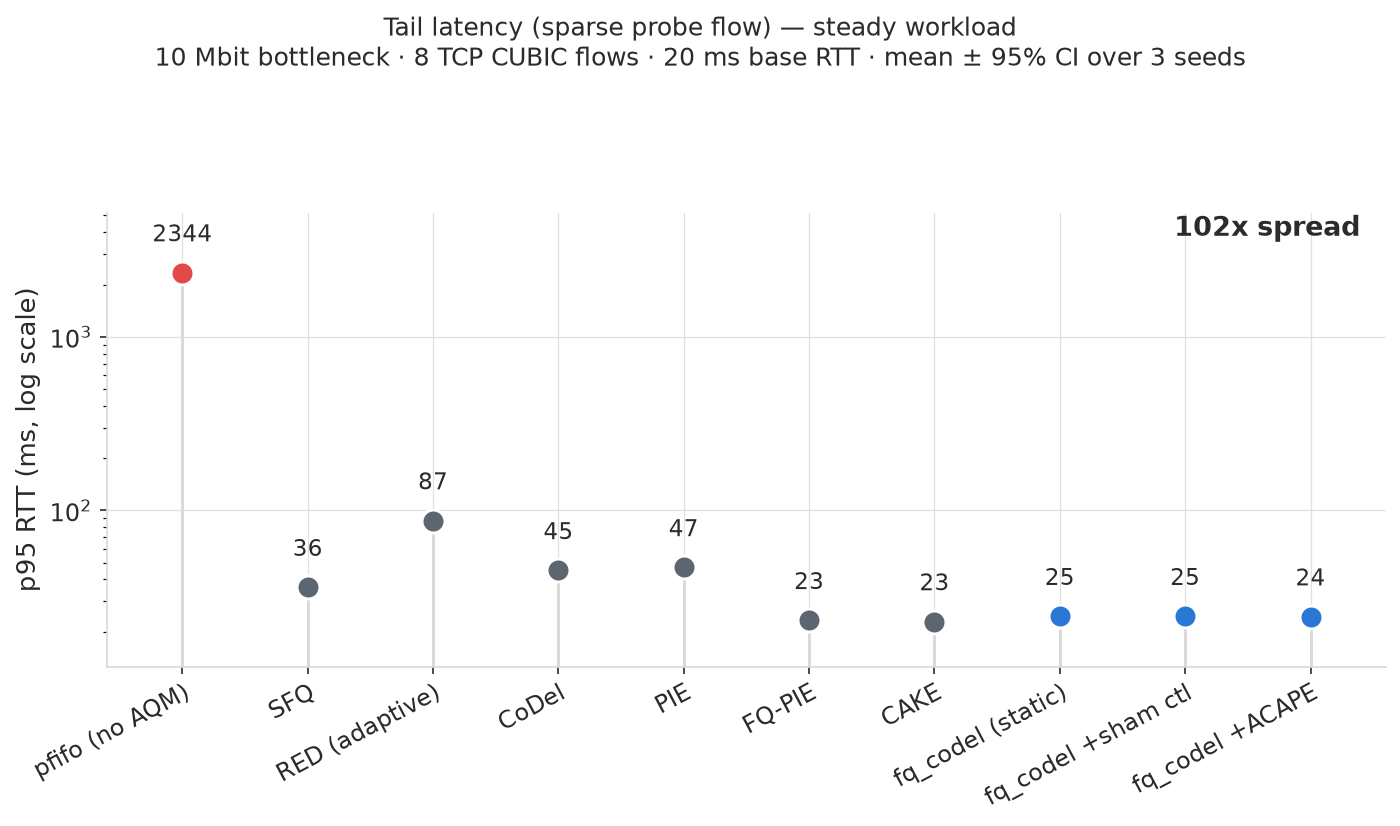
\includegraphics[width=\columnwidth]{fig01_latency_tail_steady.png}
\caption{Tail latency across all systems (log scale).}
\label{fig:fig01_latency_tail_steady}
\end{figure}

\begin{figure}[h]
\centering
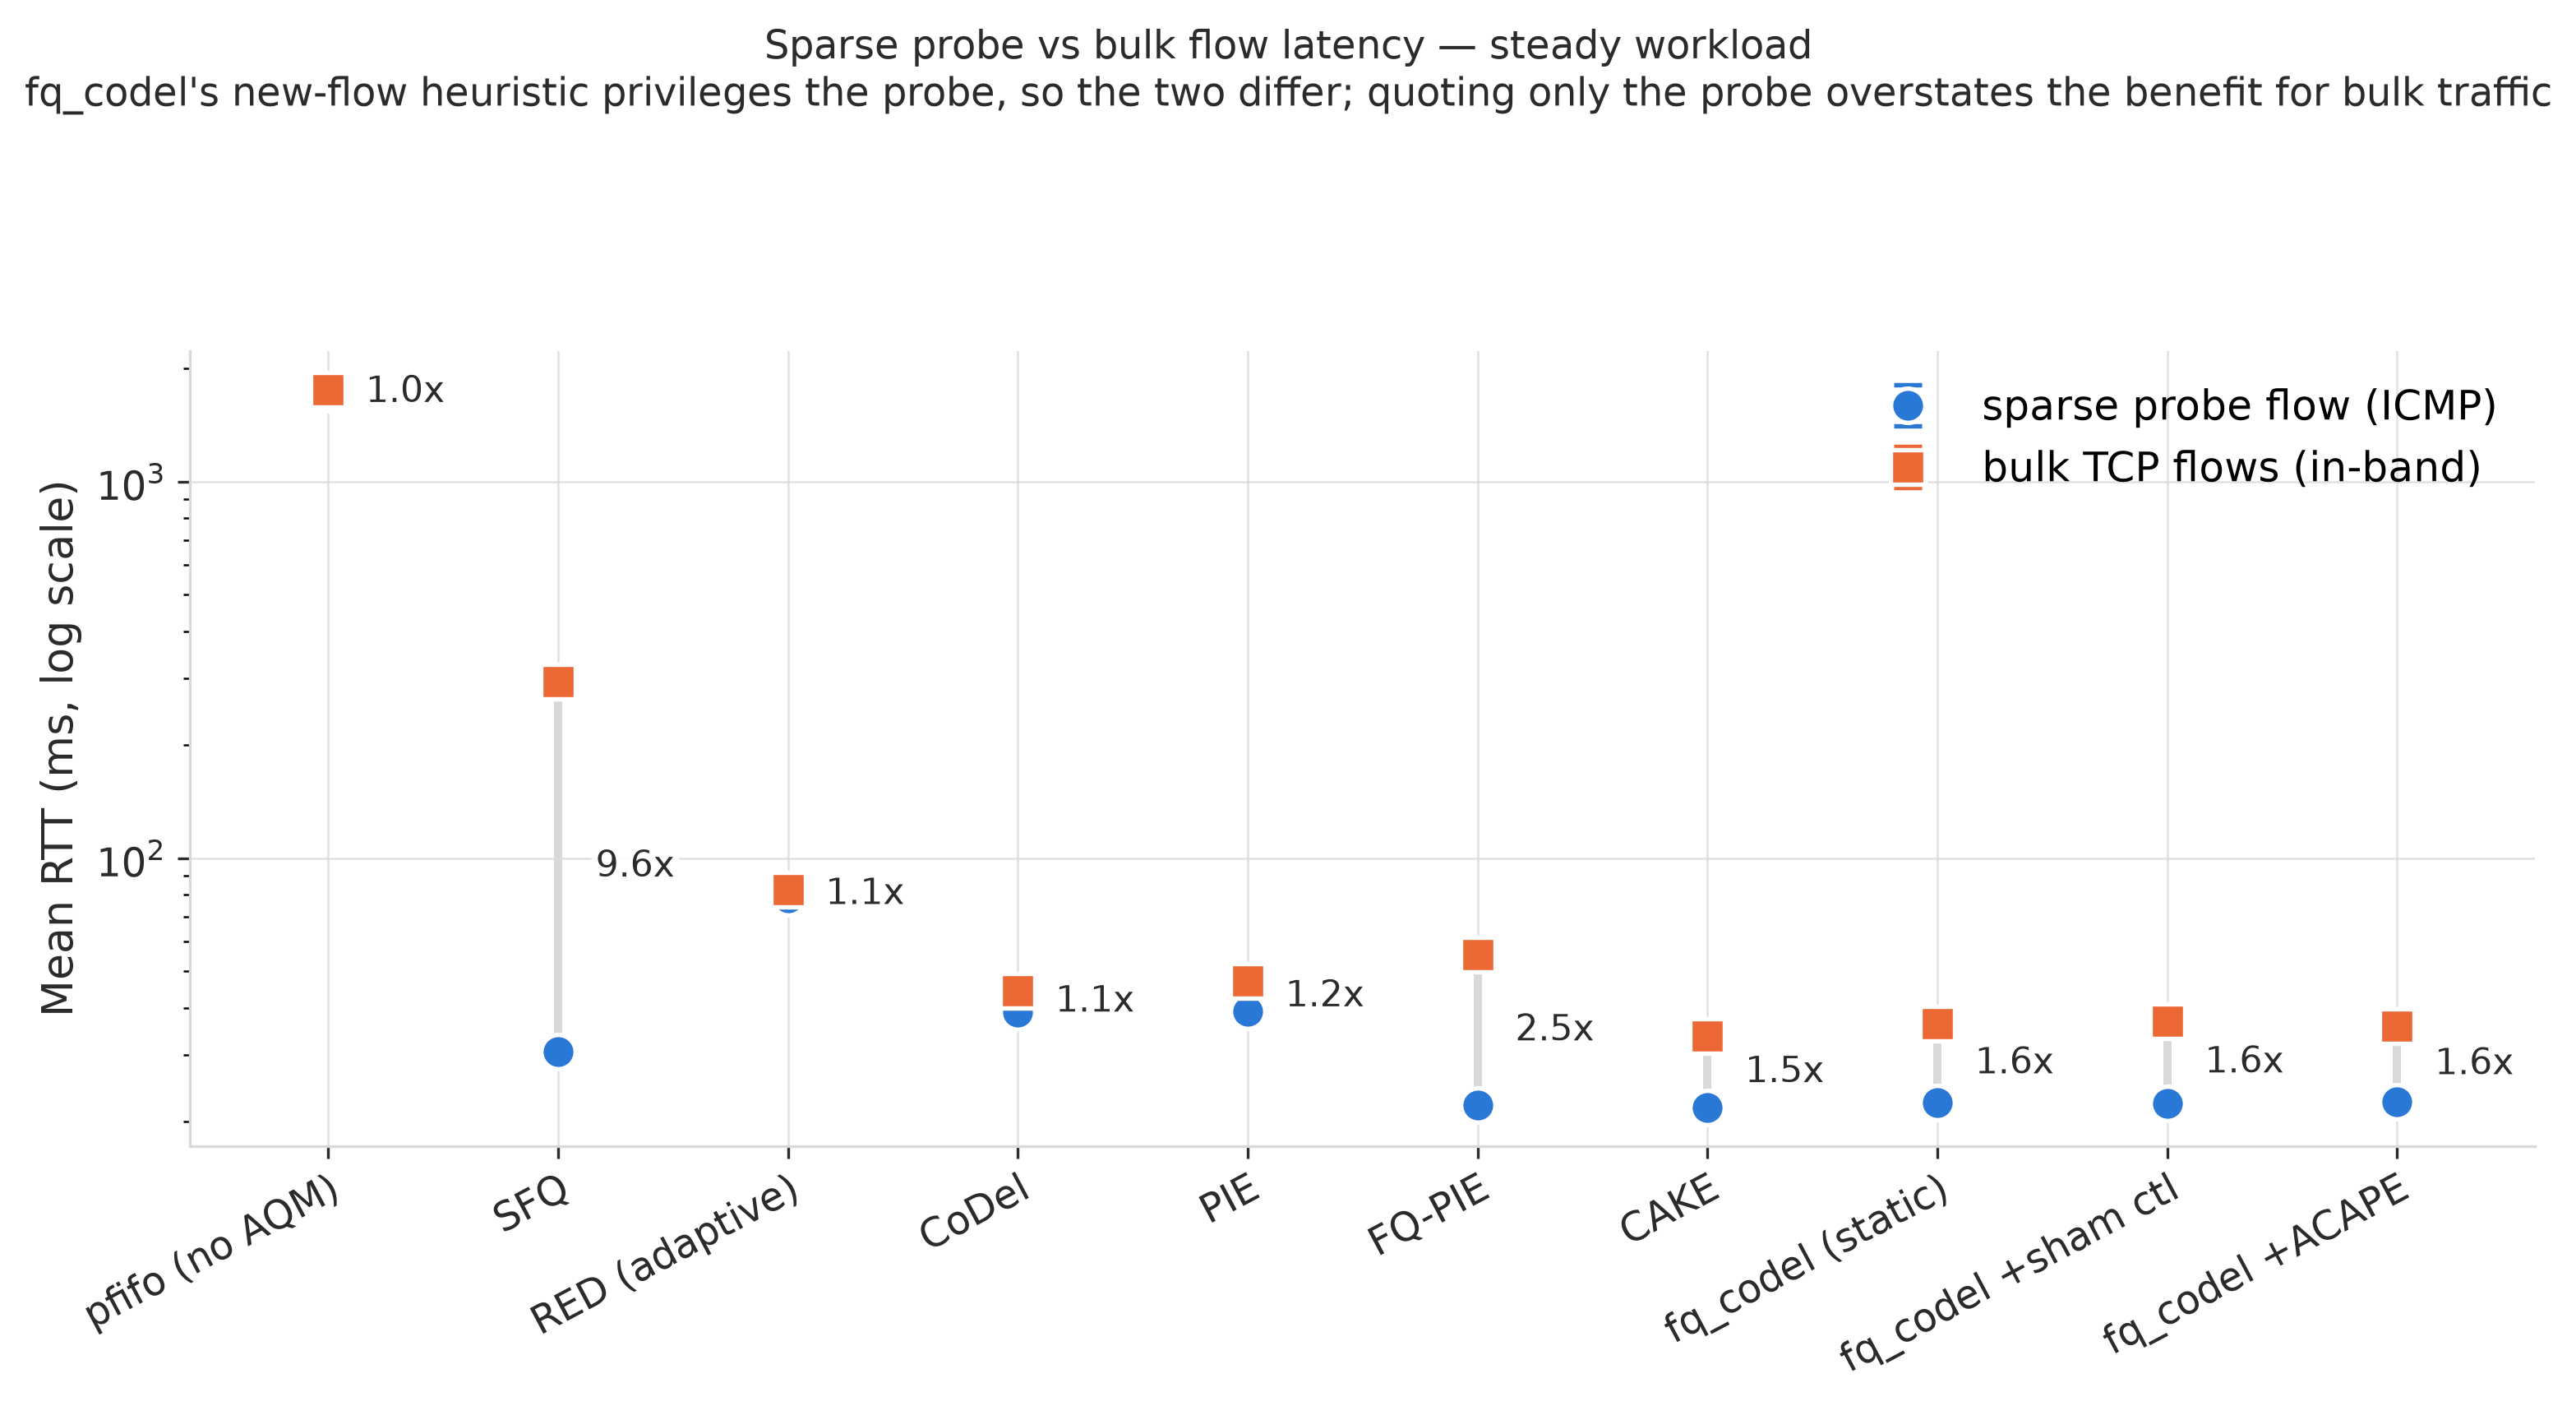
\includegraphics[width=\columnwidth]{fig02_latency_sparse_vs_bulk_steady.png}
\caption{Sparse probe flow versus bulk TCP flow RTT. The new-flow heuristic privileges the probe, so the two differ substantially.}
\label{fig:fig02_latency_sparse_vs_bulk_steady}
\end{figure}

\begin{figure}[h]
\centering
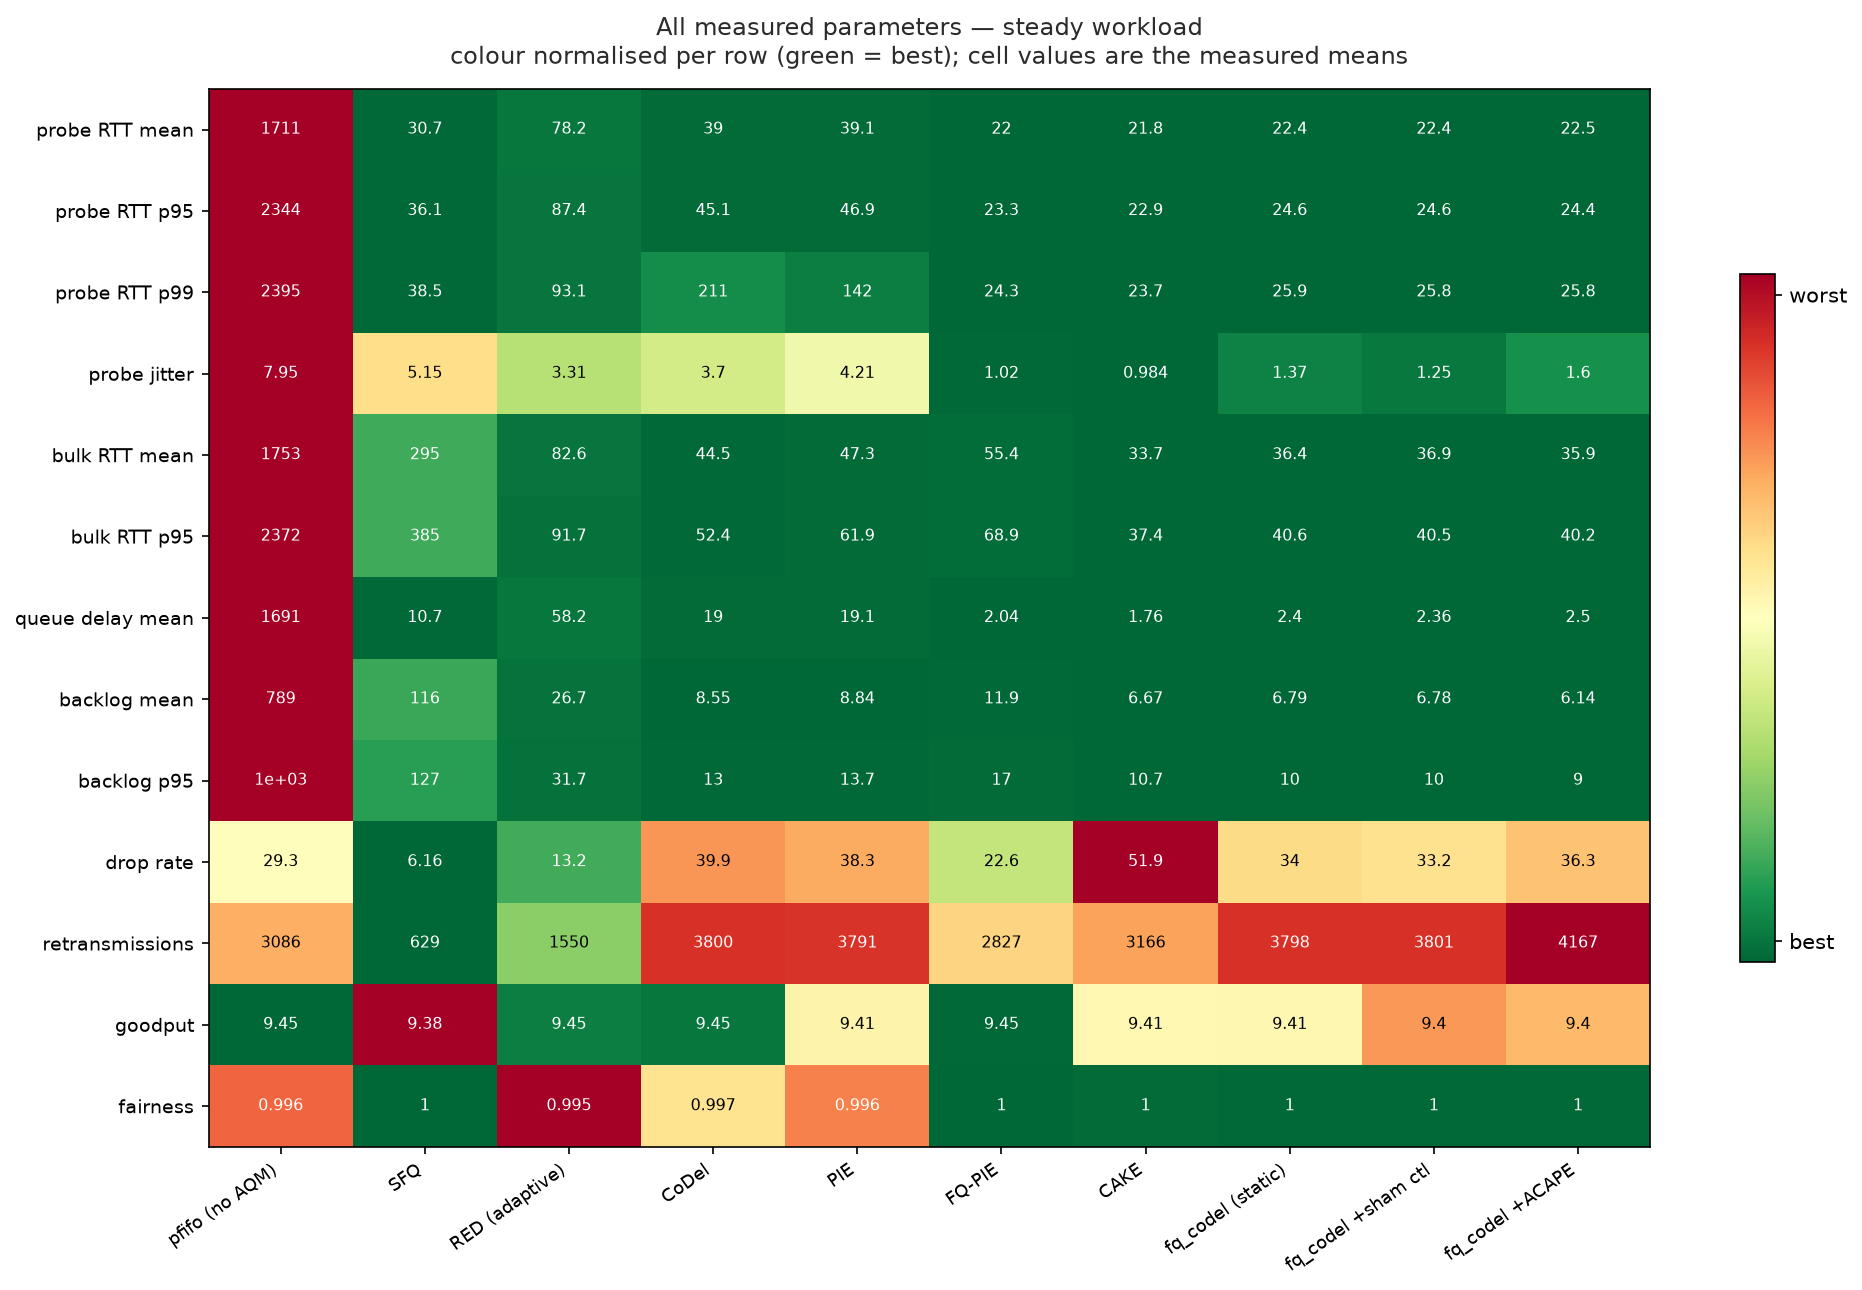
\includegraphics[width=\columnwidth]{fig08_allparams_steady.png}
\caption{Every measured parameter against every system, normalised per row; cell values are the measured means.}
\label{fig:fig08_allparams_steady}
\end{figure}

\subsection{Staged workload}

\begin{table}[h]
\centering
\scriptsize
\caption{All systems, staged workload (mean $\pm$ 95\% CI over repetitions).}
\label{tab:staged}
% GENERATED by src/analyse.py -- do not edit by hand.
\begin{tabular}{lrrrrrr}
\toprule
\textbf{System} & \textbf{Goodput} (Mbps) & \textbf{Probe RTT} (ms) & \textbf{Probe p95} (ms) & \textbf{Bulk RTT} (ms) & \textbf{Backlog} (pkt) & \textbf{Jain} \\
\midrule
pfifo (no AQM) & 8.38\,$\pm$\,0.46 & 1152.9\,$\pm$\,29.0 & 2318.0\,$\pm$\,48.9 & 1585.6\,$\pm$\,31.7 & 570.2\,$\pm$\,39.5 & 0.9862\,$\pm$\,0.0071 \\
SFQ & 9.26\,$\pm$\,0.31 & 32.8\,$\pm$\,0.5 & 56.6\,$\pm$\,3.4 & 285.6\,$\pm$\,6.1 & 96.5\,$\pm$\,8.7 & 0.9969\,$\pm$\,0.0094 \\
RED (adaptive) & 9.25\,$\pm$\,0.11 & 62.5\,$\pm$\,0.8 & 94.2\,$\pm$\,0.4 & 88.9\,$\pm$\,0.7 & 21.8\,$\pm$\,1.2 & 0.9818\,$\pm$\,0.0097 \\
CoDel & 9.28\,$\pm$\,0.06 & 55.0\,$\pm$\,4.0 & 172.0\,$\pm$\,99.1 & 105.5\,$\pm$\,4.0 & 24.1\,$\pm$\,2.1 & 0.9911\,$\pm$\,0.0081 \\
PIE & 9.22\,$\pm$\,0.06 & 40.4\,$\pm$\,2.8 & 48.6\,$\pm$\,5.4 & 119.2\,$\pm$\,53.5 & 10.3\,$\pm$\,1.0 & 0.9614\,$\pm$\,0.0291 \\
FQ-PIE & 9.22\,$\pm$\,0.06 & 21.9\,$\pm$\,0.1 & 23.2\,$\pm$\,0.1 & 101.8\,$\pm$\,3.0 & 18.6\,$\pm$\,0.8 & 0.9999\,$\pm$\,0.0004 \\
CAKE & 9.24\,$\pm$\,0.09 & 21.5\,$\pm$\,0.3 & 22.3\,$\pm$\,0.1 & 30.1\,$\pm$\,0.5 & 10.5\,$\pm$\,3.3 & 1.0000\,$\pm$\,0.0000 \\
fq\_codel (static) & 9.24\,$\pm$\,0.01 & 21.9\,$\pm$\,0.1 & 23.4\,$\pm$\,0.2 & 52.0\,$\pm$\,1.4 & 11.3\,$\pm$\,1.2 & 1.0000 \\
fq\_codel + sham ctl & 9.19\,$\pm$\,0.08 & 22.1\,$\pm$\,0.6 & 23.5\,$\pm$\,0.2 & 51.7\,$\pm$\,0.7 & 11.5\,$\pm$\,2.6 & 1.0000 \\
fq\_codel + ACAPE & 9.18\,$\pm$\,0.10 & 22.2\,$\pm$\,0.4 & 24.2\,$\pm$\,0.8 & 51.7\,$\pm$\,0.3 & 11.5\,$\pm$\,1.2 & 0.9999\,$\pm$\,0.0005 \\
\bottomrule
\end{tabular}

\end{table}

\begin{figure}[h]
\centering
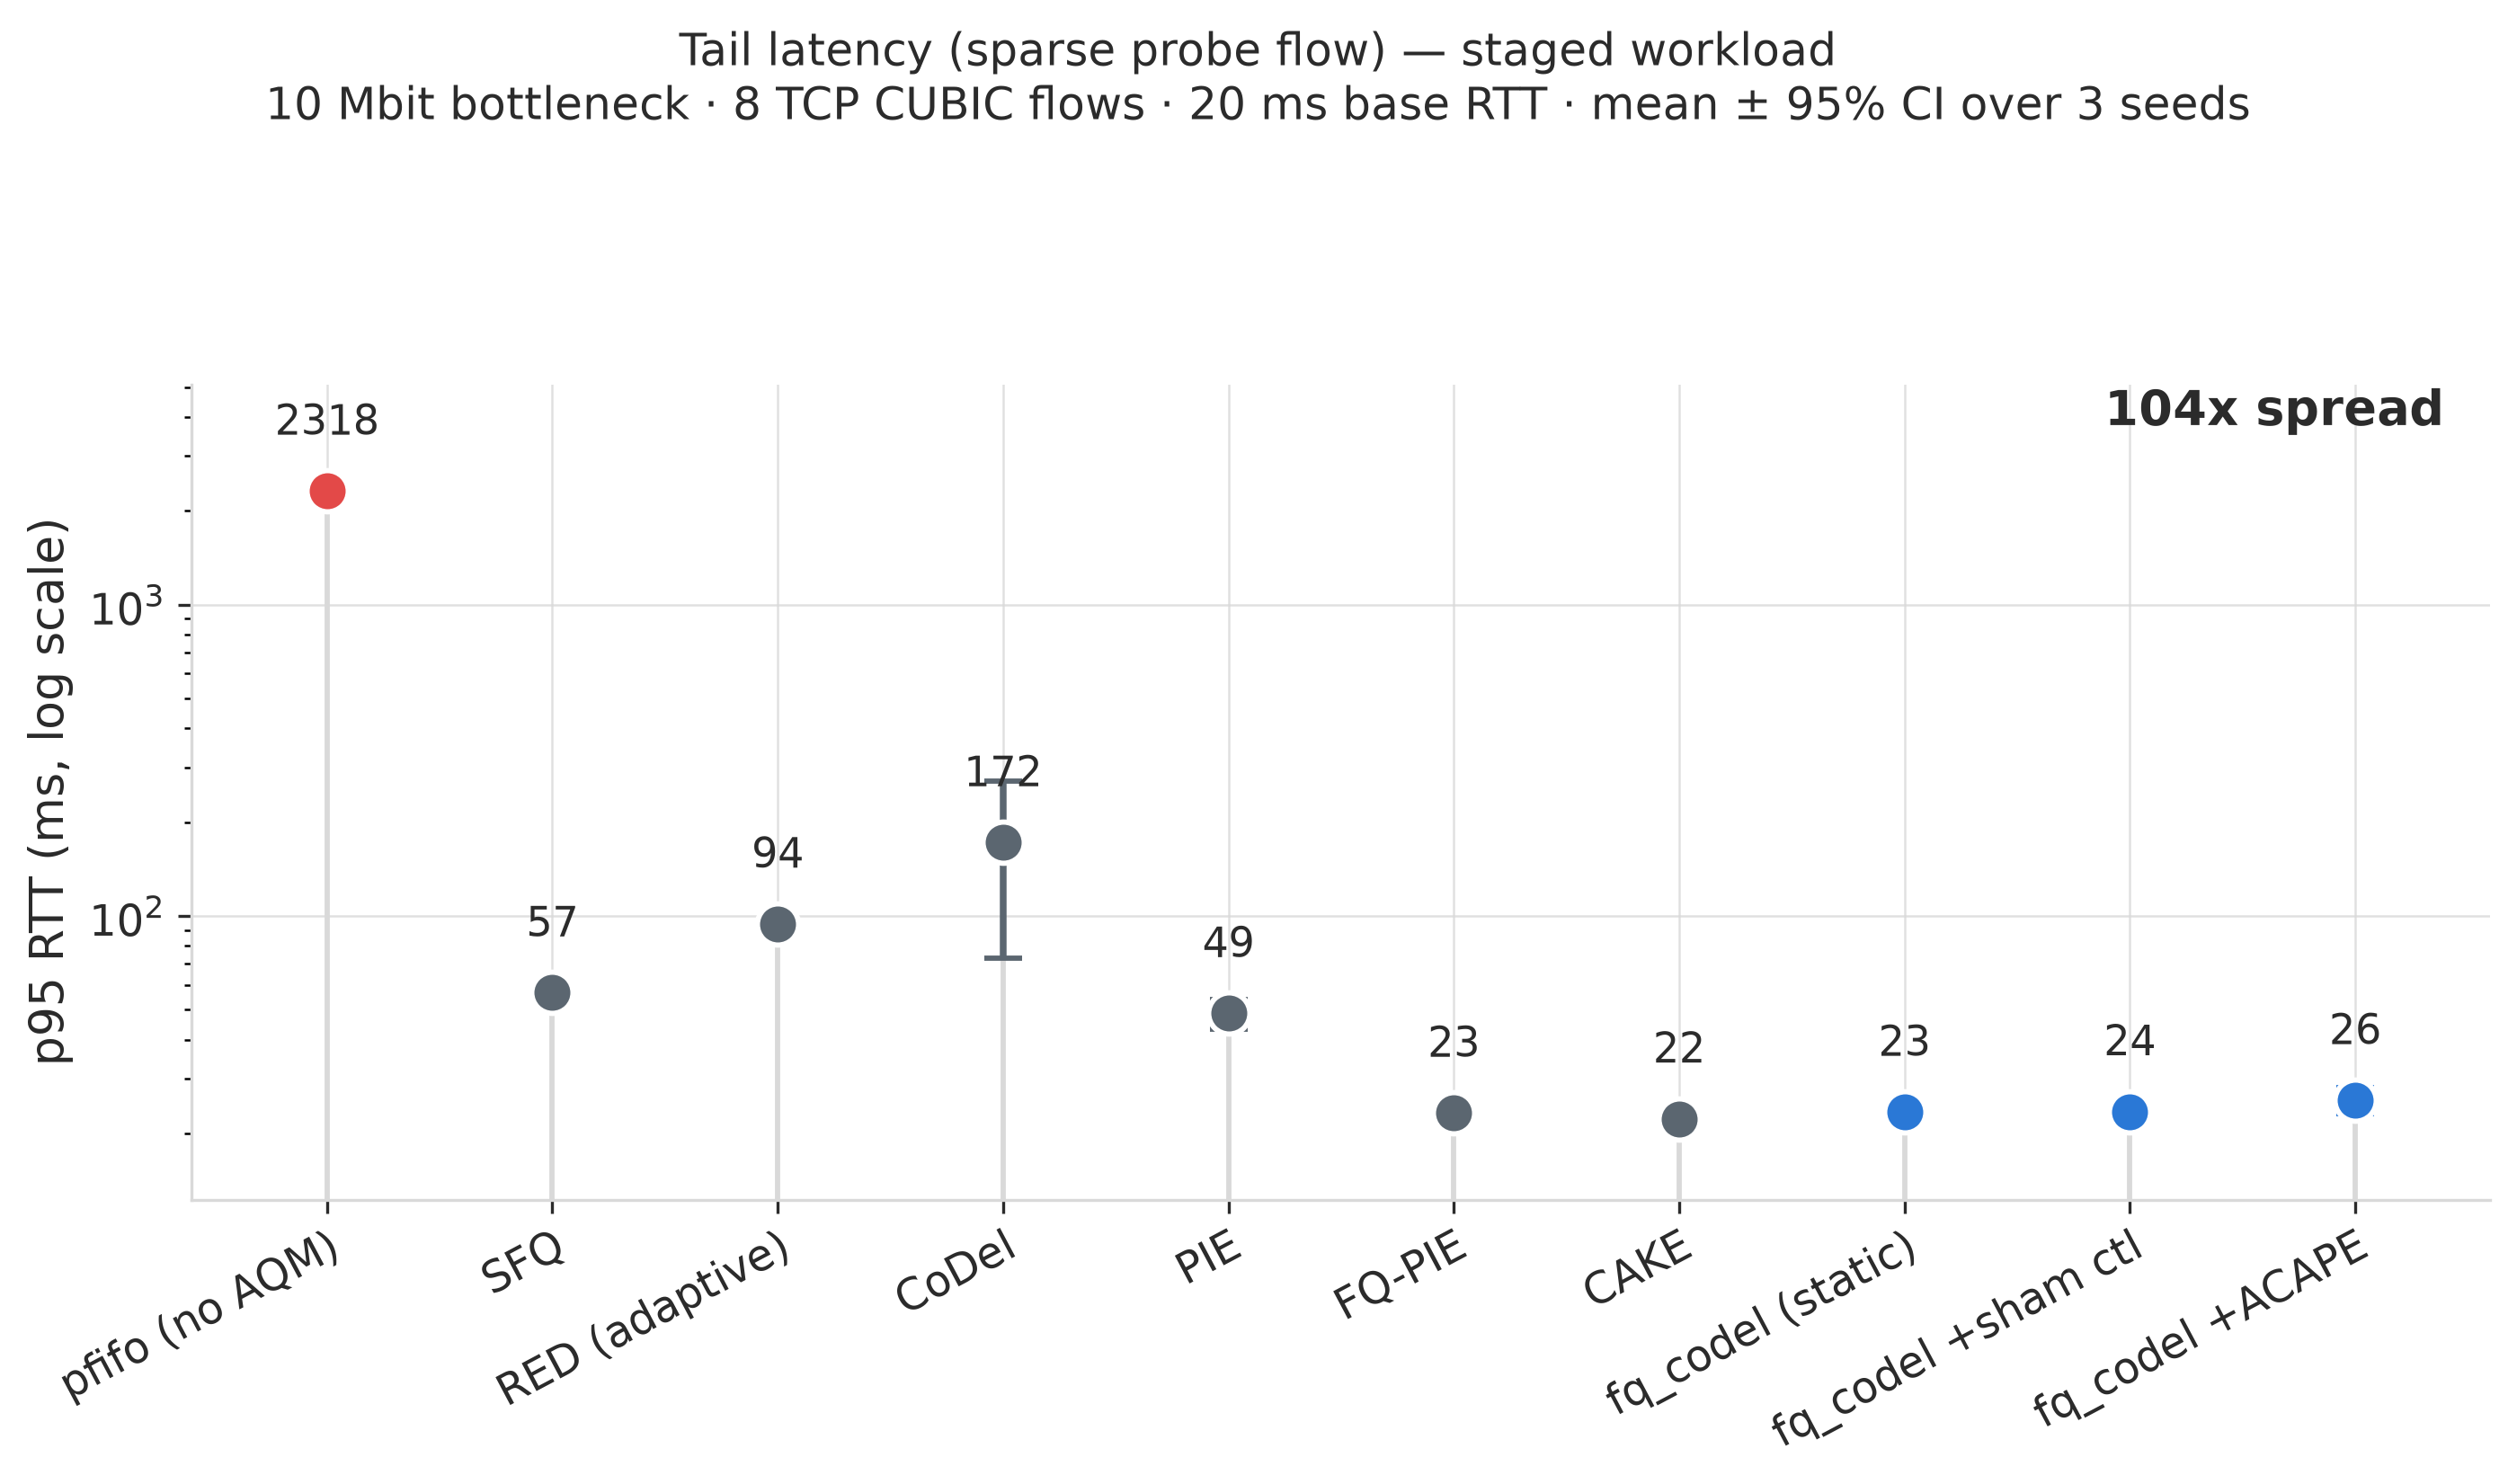
\includegraphics[width=\columnwidth]{fig01_latency_tail_staged.png}
\caption{Tail latency across all systems (log scale).}
\label{fig:fig01_latency_tail_staged}
\end{figure}

\begin{figure}[h]
\centering
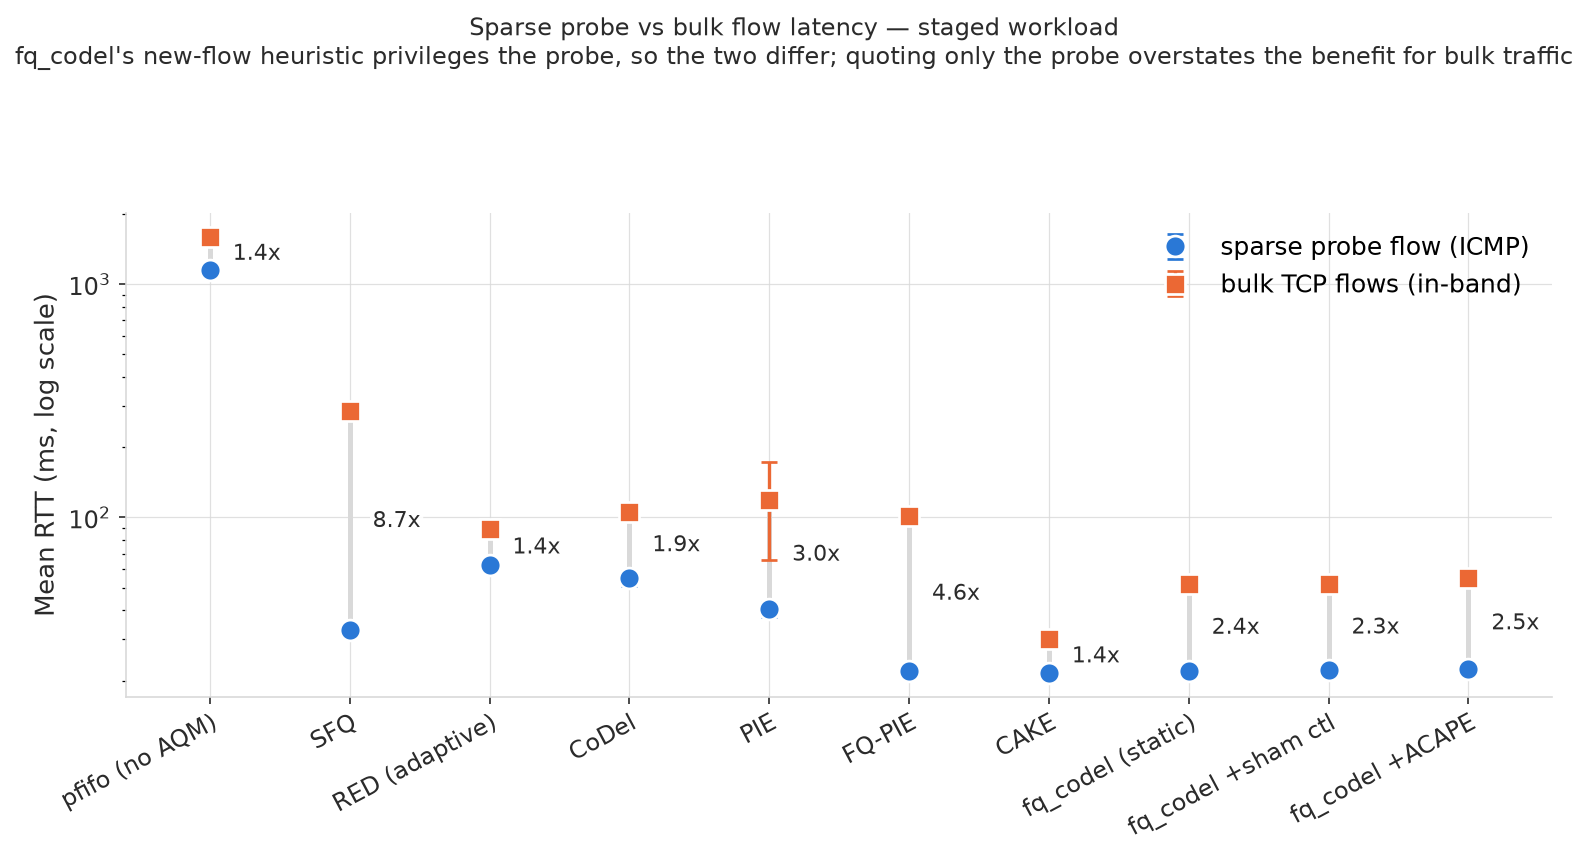
\includegraphics[width=\columnwidth]{fig02_latency_sparse_vs_bulk_staged.png}
\caption{Sparse probe flow versus bulk TCP flow RTT. The new-flow heuristic privileges the probe, so the two differ substantially.}
\label{fig:fig02_latency_sparse_vs_bulk_staged}
\end{figure}

\begin{figure}[h]
\centering
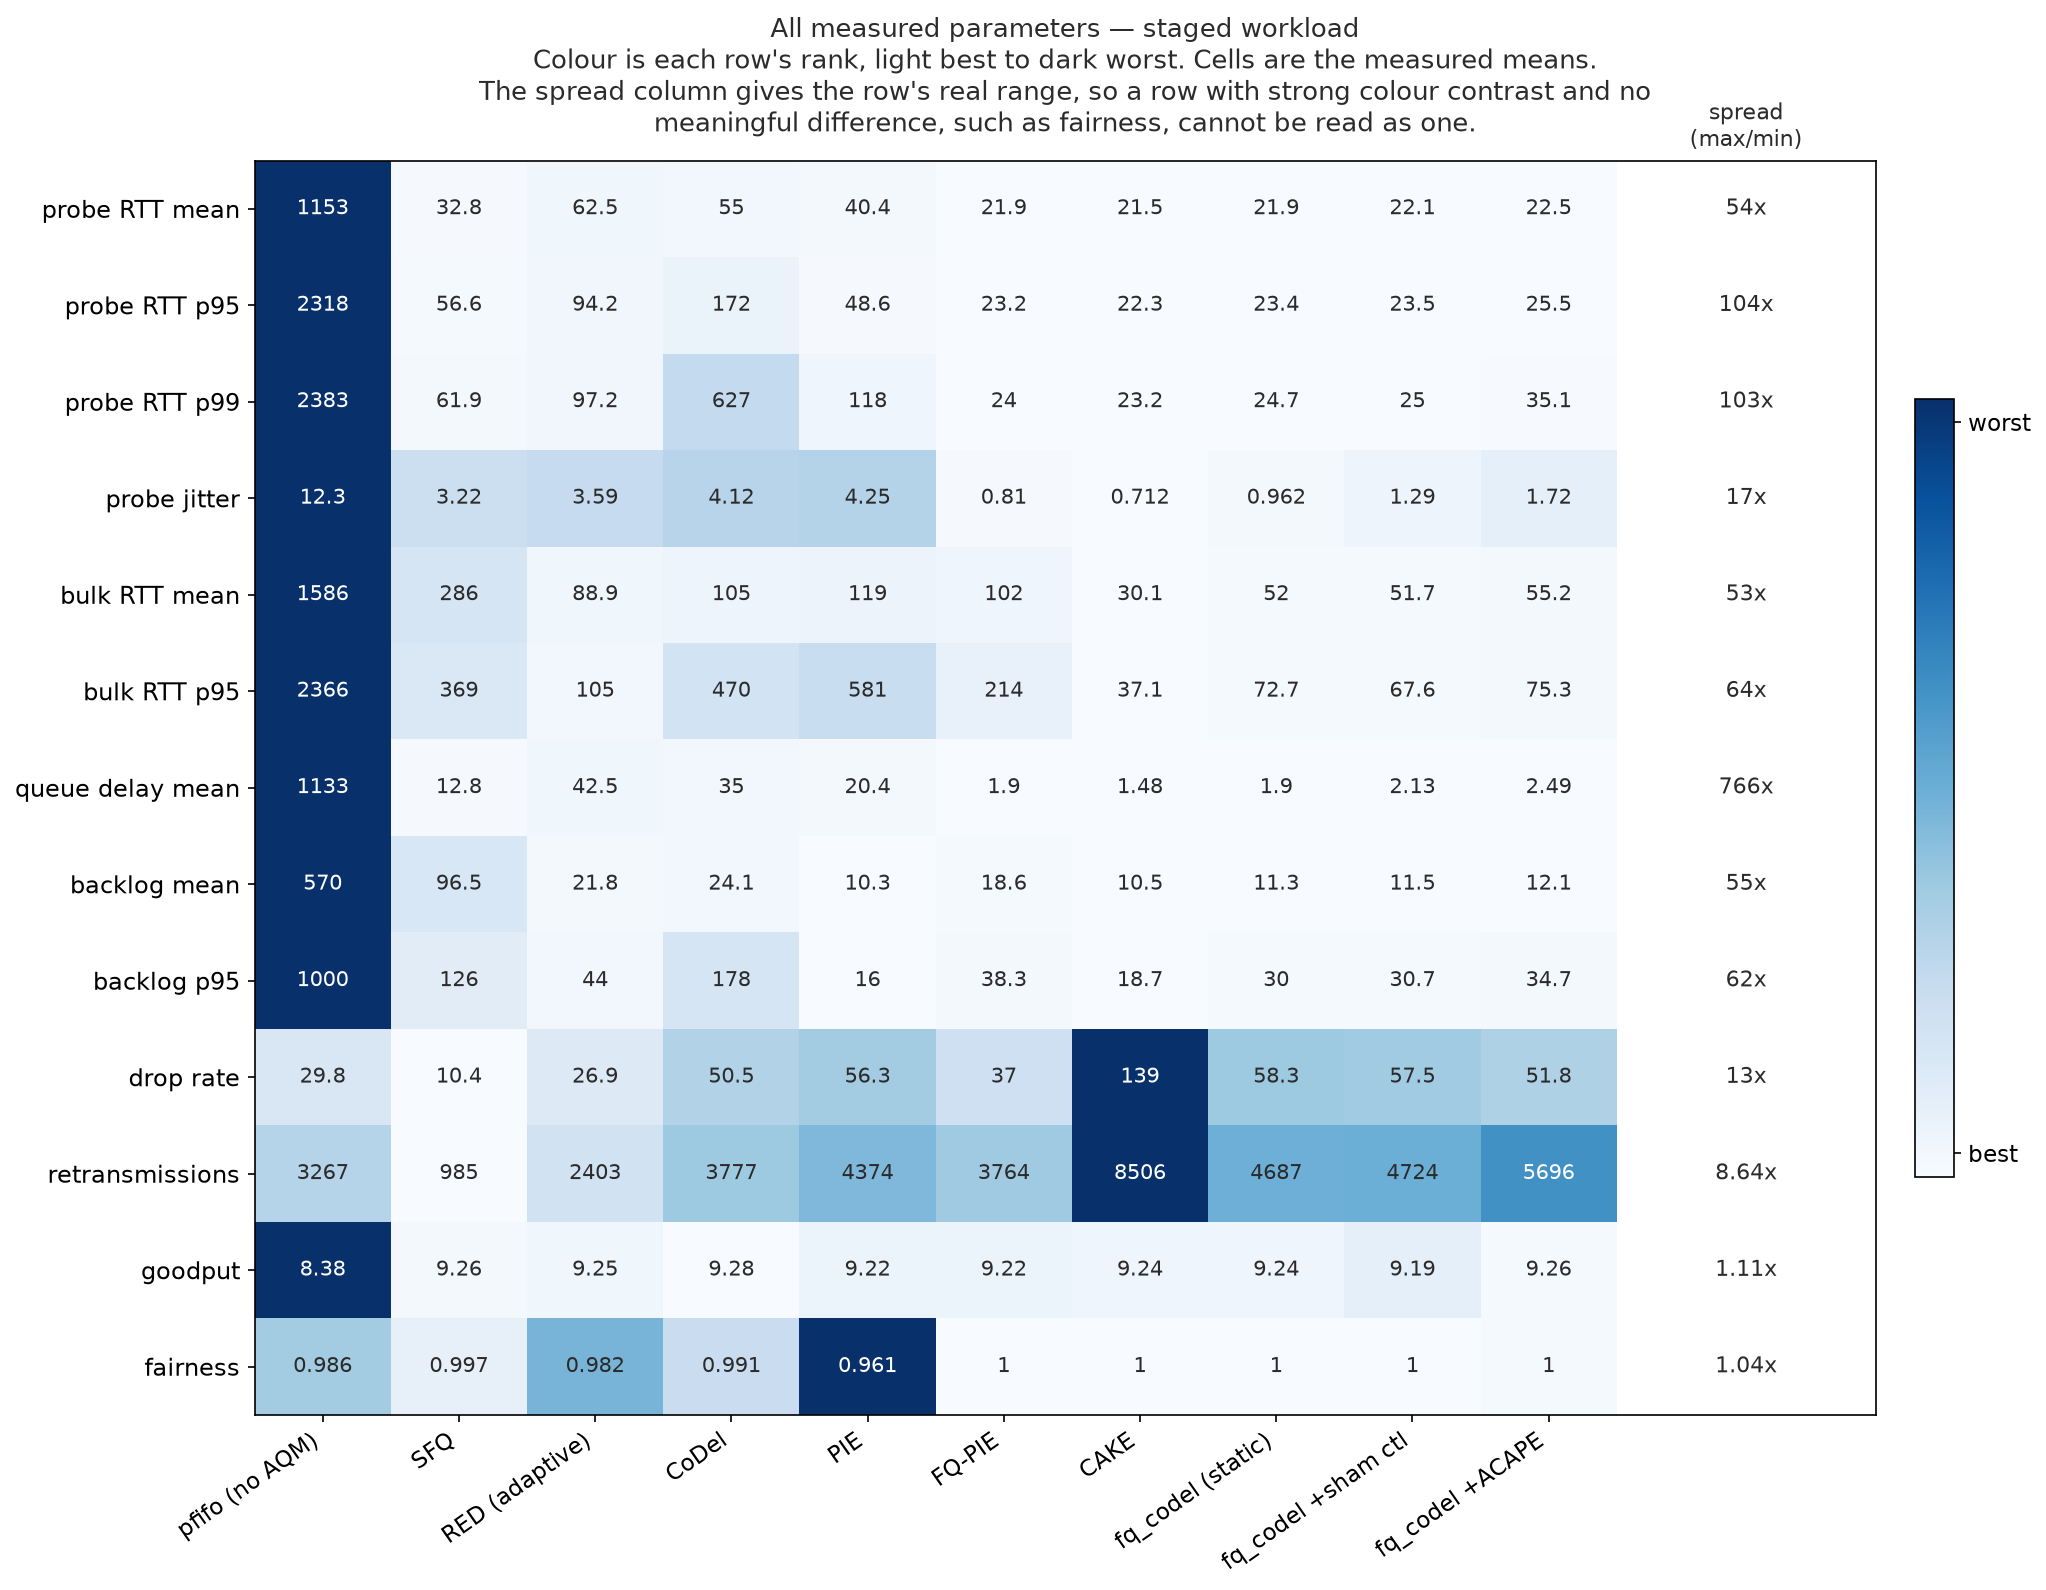
\includegraphics[width=\columnwidth]{fig08_allparams_staged.png}
\caption{Every measured parameter against every system, normalised per row; cell values are the measured means.}
\label{fig:fig08_allparams_staged}
\end{figure}



%% ============================================================
\section{Measurement Pitfalls}
\label{sec:pitfalls}

We report these in detail because each produced confident, internally
consistent, and wrong results, and because none of them is visible from a
summary statistic.

\subsection{The acknowledgement-path bottleneck}

Described in Section~\ref{sec:topology}. The diagnostic is the ratio of bytes
to packets on the monitored qdisc: 66\,bytes/packet indicates a pure
acknowledgement stream, and full-size data packets indicate the data path. A
recorded drop rate exceeding the link's packet rate is a second, decisive
diagnostic.

\subsection{Silent failure of an eBPF telemetry path}

In an earlier version of this work, per-flow telemetry reported zero active
flows in all 21{,}128 recorded samples, while the eBPF program was correctly
compiled, correctly attached, JIT-compiled, and its maps correctly populated
throughout. Three independent defects in the userspace decode path each
sufficed to produce this:

\begin{enumerate}
\item \texttt{bpftool map dump --json} renders byte arrays as hex
      \emph{strings}. Calling \texttt{bytes()} on that list raises
      \texttt{TypeError}, which a bare \texttt{except:\ pass} discarded.
\item The assumed C struct layout omitted one \texttt{u64} field, so every
      field after it was read at the wrong offset; the elephant flag was read
      from the low half of the inter-packet gap.
\item Flow age was computed by subtracting \texttt{bpf\_ktime\_get\_ns()}
      (CLOCK\_MONOTONIC) from \texttt{time.time\_ns()} (CLOCK\_REALTIME),
      yielding ages of approximately 56.8 years, so an \texttt{age < 2\,s}
      filter never matched.
\end{enumerate}

The downstream effect was that the elephant ratio was always 0, the workload
profile always MICE, and \texttt{quantum} always 300\,bytes. An earlier draft
cited that constant \texttt{quantum} as evidence the pipeline was working. It
was the signature of the failure.

The failure was originally attributed to namespace file-descriptor isolation.
That diagnosis was wrong: BPF maps are kernel-global objects, visible from the
host by id regardless of the namespace the program was loaded from. We verify
this directly (Fig.~\ref{fig:ebpf}).

\begin{figure}[t]
\centering
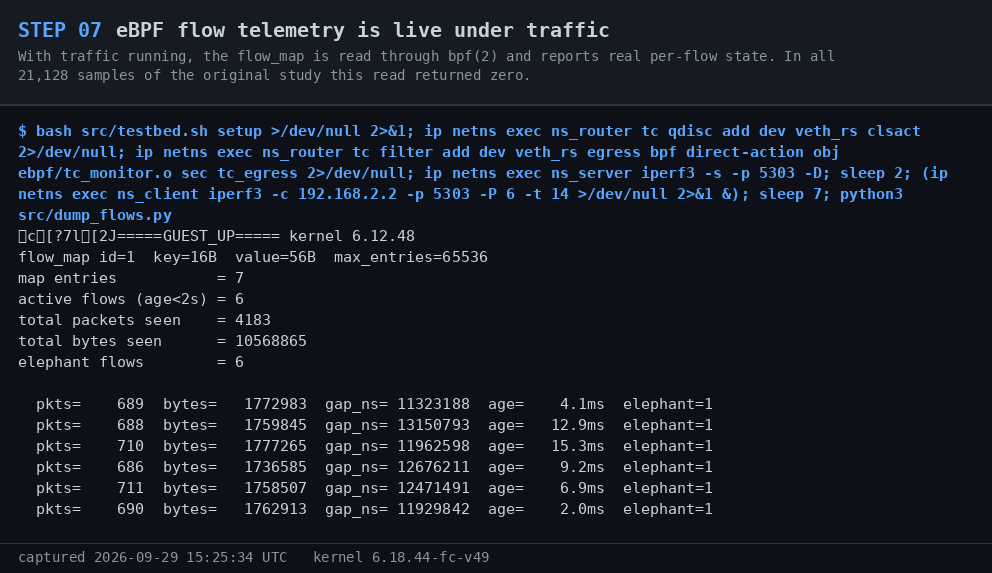
\includegraphics[width=\columnwidth]{step07_ebpf_flow_telemetry_is_live_under_traffic.png}
\caption{Live \texttt{flow\_map} contents read through \texttt{bpf(2)} under
traffic. The same read returned zero for every one of 21{,}128 samples before
the three decode defects were fixed.}
\label{fig:ebpf}
\end{figure}

\subsection{Control state that cannot reach the kernel}

The controller's internal \texttt{target} was a float, but
\texttt{tc qdisc change} was invoked with \texttt{int(round(target))}
milliseconds and the applied value was never read back. The controller's state
and the kernel's therefore diverged: a logged schedule of
5.00, 4.50, 4.05, \dots, 1.03\,ms reached the kernel as
5, 4, 4, 4, 3, 3, 3, 2, 2, 2, 2, 2, 1, 1, 1, 1\,ms. Reading parameters back
after every write is the remedy, and it is cheap.

\subsection{A control signal with no effect}

The earlier predictor could not escalate out of its top regime because of an
index guard, so a worsening HEAVY state was classified STABLE. Separately, the
effective regime was computed as the prediction only under a condition that
could never hold, so it always equalled the current regime. The consequence was
that all 375 logged adjustments applied the identical multiplicative decrease
while a subset were labelled predictive.

The general lesson is that a control input should be validated by checking that
varying it changes the output. We now assert this in a regression test:
a recovering HEAVY state and a stable HEAVY state must produce different
parameters.

\subsection{Constants that look like measurements}

The earlier work reported ``15 AIMD adjustments'' as a result. It is
$\lceil \log(1/5)/\log(0.9) \rceil$, the number of $\times 0.9$ steps from
5\,ms to a 1\,ms floor, and it appeared in 24 of 32 runs because the controller
drove to the floor and stopped in every one. Under a saturating workload the
adaptive logic was never exercised; the congestion regime was HEAVY for 80.9\%
of samples and MODERATE for 0.04\%. A four-state classifier that occupies two
states is not classifying. This is why the present work uses a staged workload
in which the flow count changes during the run.

%% ============================================================
\section{Threats to Validity}

\textbf{Emulation.} Experiments run under QEMU without hardware
virtualisation. We validated that TBF shaping is accurate under emulation
before collecting results, and absolute latencies at 20\,ms base RTT are
dominated by the configured \texttt{netem} delay rather than by host timing
jitter. Results at much higher link rates, where per-packet processing time
matters, would need re-validation.

\textbf{Scale.} A 10\,Mbit bottleneck with 8--24 flows is representative of a
home or access link, not of a datacentre or backbone. SCRR \cite{scrr2025} and
QueuePilot \cite{queuepilot2023} both address regimes we do not test.

\textbf{Traffic model.} All flows are bulk TCP CUBIC. Mixed workloads with
sparse latency-sensitive flows are exactly where \texttt{fq\_codel}'s new-flow
heuristic is designed to help, and where an adaptive \texttt{quantum} might
plausibly matter; we did not test them, and our negative result should not be
extrapolated there.

\textbf{Single bottleneck.} Multi-hop topologies with several congested links
are not covered.

%% ============================================================
\section{Conclusion}

We set out to determine whether adapting \texttt{fq\_codel}'s four parameters at
runtime improves on its defaults, and built the apparatus to answer it: a
testbed with the bottleneck on the data path, a working eBPF flow-telemetry
pipeline, and a controller applying Adaptive RED's AIMD policy under a
gradient-based trajectory estimate.

The measured answer, under the conditions we tested, is that it does not. The
dominant effect by two orders of magnitude is the presence or absence of flow
queueing with a delay-targeting AQM, not the tuning of that AQM's parameters.
This is consistent with CoDel's authors' position that its defaults are
RTT-relative by construction.

We think the more useful contribution is the methodological one. Each of the
pitfalls in Section~\ref{sec:pitfalls} produced results that were confident,
internally consistent and wrong, and each was caught only by checking a
physical invariant -- bytes per packet, the link's maximum packet rate, whether
a control input changes its output -- rather than by inspecting a summary
statistic. We suggest those checks as routine practice, and we release the full
artefact so that our own numbers can be subjected to them.

\section*{Reproducibility}

All code, kernel configuration, logs and analysis are available at
\url{https://github.com/Amritha902/ccn-linux-qdisc-study}. Every table and
every inline figure in this paper is generated directly from the experiment
logs by \texttt{src/analyse.py}; none is typed by hand.

%% ============================================================
\begin{thebibliography}{00}

\bibitem{gettys2012}
J.~Gettys and K.~Nichols, ``Bufferbloat: Dark Buffers in the Internet,''
\textit{Commun. ACM}, vol.~55, no.~1, pp.~57--65, Jan. 2012.

\bibitem{red1993}
S.~Floyd and V.~Jacobson, ``Random Early Detection Gateways for Congestion
Avoidance,'' \textit{IEEE/ACM Trans. Netw.}, vol.~1, no.~4, pp.~397--413,
Aug. 1993.

\bibitem{ared2001}
S.~Floyd, R.~Gummadi, and S.~Shenker, ``Adaptive RED: An Algorithm for
Increasing the Robustness of RED's Active Queue Management,'' ICSI Technical
Report, Aug. 2001.

\bibitem{nichols2012}
K.~Nichols and V.~Jacobson, ``Controlling Queue Delay,'' \textit{ACM Queue},
vol.~10, no.~5, pp.~20--34, May 2012.

\bibitem{rfc8289}
K.~Nichols, V.~Jacobson, A.~McGregor, and J.~Iyengar, ``Controlled Delay Active
Queue Management,'' IETF RFC 8289, Jan. 2018.

\bibitem{rfc8290}
T.~H\o{}iland-J\o{}rgensen, P.~McKenney, D.~T\"{a}ht, J.~Gettys, and
E.~Dumazet, ``The FlowQueue-CoDel Packet Scheduler and Active Queue Management
Algorithm,'' IETF RFC 8290, Jan. 2018.

\bibitem{rfc8033}
R.~Pan, P.~Natarajan, F.~Baker, and G.~White, ``Proportional Integral Controller
Enhanced (PIE): A Lightweight Control Scheme to Address the Bufferbloat
Problem,'' IETF RFC 8033, Feb. 2017.

\bibitem{fqpie2019}
G.~Ramakrishnan, M.~Bhasi, V.~Saicharan, L.~Monis, S.~D.~Patil, and
M.~P.~Tahiliani, ``FQ-PIE Queue Discipline in the Linux Kernel: Design,
Implementation and Challenges,'' in \textit{Proc. IEEE LCN Symp.}, Oct. 2019.

\bibitem{cake2018}
T.~H\o{}iland-J\o{}rgensen, D.~T\"{a}ht, and J.~Morton, ``Piece of CAKE: A
Comprehensive Queue Management Solution for Home Gateways,'' in
\textit{Proc. IEEE LANMAN}, Jun. 2018.

\bibitem{scrr2025}
E.~Sharafzadeh, R.~Matson, J.~Tourrilhes, P.~Sharma, and S.~Ghorbani,
``Self-Clocked Round-Robin Packet Scheduling,'' in \textit{Proc. USENIX NSDI},
Apr. 2025.

\bibitem{desired2024}
F.~Rodriguez et al., ``DESiRED --- Dynamic, Enhanced, and Smart iRED: A P4-AQM
with Deep Reinforcement Learning and In-band Network Telemetry,''
\textit{Computer Networks}, vol.~244, 2024.

\bibitem{aqmllm2026}
D.~Satish et al., ``Distilling Large Language Models for Network Active Queue
Management,'' \textit{IEEE Trans. Netw.}, 2026.

\bibitem{queuepilot2023}
M.~Dery, O.~Krupnik, and I.~Keslassy, ``QueuePilot: Reviving Small Buffers With
a Learned AQM Policy,'' in \textit{Proc. IEEE INFOCOM}, 2023.

\bibitem{mlaqm2025}
M.~P.~Toopchinezhad and M.~Ahmadi, ``Machine Learning Approaches for Active
Queue Management: A Survey, Taxonomy, and Future Directions,''
\textit{Computer Networks}, vol.~262, May 2025.

\bibitem{yeleung2020}
J.~Ye and K.-C.~Leung, ``Adaptive and Stable Delay Control for Combating
Bufferbloat: Theory and Algorithms,'' \textit{IEEE Systems Journal}, vol.~14,
no.~1, pp.~1285--1296, Mar. 2020.

\bibitem{rfc9330}
B.~Briscoe, K.~De~Schepper, M.~Bagnulo, and G.~White, ``Low Latency, Low Loss,
and Scalable Throughput (L4S) Internet Service: Architecture,'' IETF RFC 9330,
Jan. 2023.

\bibitem{rfc9332}
K.~De~Schepper, B.~Briscoe, and G.~White, ``Dual-Queue Coupled Active Queue
Management (AQM) for Low Latency, Low Loss, and Scalable Throughput (L4S),''
IETF RFC 9332, Jan. 2023.

\bibitem{cubic2008}
S.~Ha, I.~Rhee, and L.~Xu, ``CUBIC: A New TCP-Friendly High-Speed TCP
Variant,'' \textit{ACM SIGOPS Oper. Syst. Rev.}, vol.~42, no.~5, pp.~64--74,
2008.

\bibitem{borkar1997}
V.~S.~Borkar, ``Stochastic Approximation with Two Time Scales,''
\textit{Syst. Control Lett.}, vol.~29, no.~5, pp.~291--294, 1997.

\bibitem{jain1984}
R.~Jain, D.-M.~Chiu, and W.~Hawe, ``A Quantitative Measure of Fairness and
Discrimination for Resource Allocation in Shared Computer Systems,'' DEC
Research Report TR-301, Sep. 1984.

\bibitem{vieira2020}
M.~A.~M.~Vieira et al., ``Fast Packet Processing with eBPF and XDP: Concepts,
Code, Challenges, and Applications,'' \textit{ACM Comput. Surv.}, vol.~53,
no.~1, Article~16, 2020.

\bibitem{rfc7567}
F.~Baker and G.~Fairhurst, ``IETF Recommendations Regarding Active Queue
Management,'' IETF RFC 7567, Jul. 2015.

\end{thebibliography}

\end{document}
